\section{Komponenten}
\label{sys_sec:Komponenten}
Folgend werden alle im Lokkit System vorhandenen Komponenten, deren Abhängigkeiten und vorgenommene Konfiguration erklärt.

\subsection{Geth}
\label{sys_subsec:Geth}
\begin{itemize}
    \item Konfiguration von Geth
    \item Funktionsweise blockchain KURZ
\end{itemize}

\subsection{Smart Contracts}
Die Datenhaltung und Businesslogik des Lokkit Systems liegt auf der Blockchain in Form von Smart Contracts.
\subsubsection{Rentable}
\label{sys_subsubsec:Rentable}
Eine Instanz dieses Contracts spiegelt ein mietbares Objekt wieder.

\paragraph{Attribute}
\label{sys_para:Rentable_Attribute}
Attribute eines Rentable können gelesen und gesetzt werden. Lesen wird durch die automatische Lesefunktion von Solidity gemacht, gesetzt werden die Attribute durch eine entsprechende Funktion, die den prefix \emph{set} hat und den neuen Wert als einzigen Parameter annimmt. Wichtig zu beachten ist, dass die Funktion zum Ändern des Owners nicht setOwner sondern \emph{transferOwnership} heisst. Dieser Name widerspiegelt die Tatsache, dass der Besitz transferiert wird und sollte nicht leichtfertig mit einer \emph{set} Funktion verwechselt werden. Wenn eine Eigenschaft mittels einer \emph{set} Funktion verändert wird, wird das OnUpdate\emph{X} Event ausgelöst, wobei X für die veränderte Eigenschaft steht. 

\begin{longtable}{@{}llL{9cm}@{}}
\caption{Rentable Eigenschaften}\label{tbl:Rentable_Eigenschaften}\\
\toprule
Name & Typ & Beschreibung \\ \midrule
owner & address   & Besitzer des Rentable Objektes. Kann Eigenschaften verändern und privilegierte Funktionen ausführen.\\
description & string   & Beschreibung des Rentable Objektes.\\
location & string   & Besitzer des Rentable Objektes. Kann Eigenschaften verändern und privilegierte Funktionen ausführen.\\
costPerSecond & uint   & Kosten des Rentables in Wei pro Sekunde.\\
deposit & uint   & Menge Wei, die hinterlegt werden muss. Wird zurückerstattet, wenn \emph{unclaim} oder \emph{forceUnclaim} aufgerufen werden (vgl. \ref{sys_para:claim_unclaim}).\\
\end{longtable}

\paragraph{Berechnung der Kosten}
Die totalen Kosten eines Rentable für einen Zeitraum werden durch zwei Faktoren bestimmt: die Kosten in wei pro Sekunde (vgl. \ref{sys_para:Rentable_Attribute}) und das zu hinterlegende Depot (vgl \ref{math:Rentable_Cost}). Sollte die überwiesene Menge Ether zu gross sein, wird der Überschuss in die \emph{pendingRefunds} (vgl. XX) der sendenden Adresse gutgeschrieben.

\begin{equation}
\label{math:Rentable_Cost}
totalCost = (rentDuration * costPerSecond) + deposit
\end{equation}

\paragraph{unclaim und forceUnclaim}
\label{sys_para:claim_unclaim}
Um die regelkonforme Rückgabe eines Rentables festzustellen, muss vom Mieter die Funktion \emph{unclaim} aufgerufen werden (vgl. \ref{tbl:Rentable_Funktionsuebersicht}). Damit bestätigt der Mieter, dass das Rentable nicht länger verwendet wird. Sollte der Mieter nicht unclaim aufrufen, kann der \emph{owner} zu einem Zeitpunkt nach der Reservation die Funktion \emph{forceUnclaim} aufrufen (vgl. \ref{tbl:Rentable_Funktionsuebersicht}), um das Depot seinen \emph{pendingRefunds} gutzuschreiben.

\paragraph{pendingRefunds}
Falls zu viel Ether an den Contract überwiesen wird oder eine Rückerstattung des \emph{deposit} erwirkt wurde, werden die Beträge in die \emph{pendungRefunds} des Rentables eingetragen. Diese können explizit aus deom Smart Contract abgehoben werden.\cite[Miscellaneous/Introduction to Smart Contracts]{solidity.readthedocs.io}

\paragraph{Funktionsübersicht}

L: Lesefunktion, S: Schreibfunktion, C: Konstruktor, E: Event

Alle Funktionen, die einen Zeitpunkt als Parameter (\emph{start} oder \emph{end}) annehmen, setzen ein Unix timestamp Format voraus.

\begin{longtable}{@{}lcL{9cm}@{}}
\caption{Rentable Lesefunktionen}\label{tbl:Rentable_Funktionsuebersicht}\\
\toprule
Name & Typ & Beschreibung \\ \midrule
allReservations     & L   & Gibt alle Reservationen als Array zurück. Eine Reservation besteht aus einem Array mit drei Einträgen: Startzeit, Endzeit, Ob die aufrufende Adresse der Mieter ist.\\
 & & Parameter: keine \\\midrule
reservedAt          & L   & Gibt zurück, ob das Rentable am gegebenen Zeitpunkt \emph{time} reserviert ist.\\ & & Parameter: \emph{time} \\\midrule
reservedBetween     & L   & Gibt zurück, ob das Rentable zwischen den gegebenen Zeitpunkten \emph{start} und \emph{end} reserviert ist.\\ & & Parameter: \emph{start}, \emph{end} \\\midrule
currentRenter       & L   & Gibt die Adresse des momentanen Mieters zurück. Wenn das Rentable momentan nicht vermietet ist, wird 0 zurückgegeben.\\ & & Parameter: keine \\\midrule
costInWei           & L   & Gibt die Kosten in Wei für die Zeit zwischen \emph{start} und \emph{end} zurück.\\ & & Parameter: \emph{start}, \emph{end} \\\midrule
myPendingRefund     & L   & Gibt zurück, wie viel Ether die aufrufende Adresse noch zur Verfügung hat.\\ & & Parameter: keine \\ \midrule
currentReservation  & L   & Gibt die momentane Reservation zurück als Array mit drei Einträgen: Startzeit, Endzeit, Ob die aufrufende Adresse der Mieter ist.\\ & & Parameter: keine \\\midrule
transferOwnership   & S   & Setzt den \emph{owner} des Rentables auf die angegebene Adresse \emph{newOwner}.\\ & & Parameter: \emph{newOwner} \\\midrule
setDescription   & S   & Setzt \emph{description} des Rentables auf den angegebenen Text \emph{newDescription}.\\ & & Parameter: \emph{newDescription} \\\midrule
setLocation   & S   & Setzt die \emph{location} des Rentables auf den angegebenen Text \emph{newLocation}.\\ & & Parameter: \emph{newLocation} \\\midrule
setCostPerSecond   & S   & Setzt die \emph{costPerSecond} des Rentables auf die angegebene Menge \emph{newCostPerSecond}.\\ & & Parameter: \emph{newCostPerSecond} \\\midrule
setDeposit   & S   & Setzt das \emph{peposit} des Rentables auf die angegebene Menge \emph{newDeposit}.\\ & & Parameter: \emph{newDeposit} \\\midrule
rent                & S   & Mietet das Rentable zwischen \emph{start} und \emph{end} für die sendende Adresse.\newline{}Vorbedingungen: start muss früher als end sein. Die Menge Ether muss für die Reservation ausreichen (vgl. \emph{costInWei}). \\ & & Parameter: \emph{start}, \emph{end} \\\midrule
unclaim         & S   & Retourniert ein Rentable während die gemietete Zeit noch nicht abgelaufen ist. Der bezahlte Betrag für die zusätzliche Zeit wird gleichmässig zwischen \emph{renter} und \emph{owner} aufgeteilt. Das \emph{deposit} wird dem refund des \emph{renter}s gutgeschrieben.\\ & & Parameter: keine \\\midrule
forceUnclaim         & S   & Retourniert alle Reservations, die in der Vergangenheit liegen und auf welchen nicht unclaim aufgerufen wurde. Das \emph{deposit} wird dem refund des \emph{owner}s gutgeschrieben.\\ & & Parameter: keine \\\midrule
withdrawRefunds     & S   & Hebt alle bestehenden Rückerstattungen einer Adresse vom Rentable ab und überweist sie auf das Konto der sendenden Adresse\\ & & Parameter: keine \\\midrule
Rentable            & C   & Erstellt ein neues Rentable mit den angegebenen Parametern und der sendenden Adresse als \emph{owner}.\\ & & Parameter: \emph{pdescription}, \emph{plocation}, \emph{pcostPerSecond}, \emph{pdeposit} \\ \midrule
OnRent              & E   & Wird ausgelöst, wenn versucht wird, das Rentable zu mieten (vgl. Funktion \emph{rent}). \emph{success} gibt an, ob die Reservation erfolgreich war. \emph{msg} beinhaltet eine Statusmeldung zum Funktionsaufruf (Fehlerbeschreibung im Fehlerfall).\\ & & Parameter: \emph{success}, \emph{renter}, \emph{start}, \emph{end}, \emph{msg} \\ \midrule
OnUpdateOwner              & E   & Wird ausgelöst, wenn \emph{owner} durch die \emph{transferOwnership} Funktion verändert wird.\\ & & Parameter: \emph{oldOwner}, \emph{newOwner} \\ \midrule
OnUpdateDescription              & E   & Wird ausgelöst, wenn \emph{description} durch die \emph{setDescription} Funktion verändert wird.\\ & & Parameter: \emph{oldDescription}, \emph{newDescription} \\ \midrule
OnUpdateLocation              & E   & Wird ausgelöst, wenn \emph{location} durch die \emph{setLocation} Funktion verändert wird.\\ & & Parameter: \emph{oldLocation}, \emph{newLocation} \\ \midrule
OnUpdateCostPerSecond              & E   & Wird ausgelöst, wenn \emph{costPerSecond} durch die \emph{setCostPerSecond} Funktion verändert wird.\\ & & Parameter: \emph{oldCostPerSecond}, \emph{newCostPerSecond} \\ \midrule
OnUpdateDeposit              & E   & Wird ausgelöst, wenn \emph{deposit} durch die \emph{setDeposit} Funktion verändert wird.\\ & & Parameter: \emph{oldDeposit}, \emph{newDeposit} \\
\bottomrule
\end{longtable}


\subsection{Webapp}
\label{sys_subsec:Webapp}

Die Webapp für Lokkit stellt eine Gerätunabhängige Benutzeroberfläche für die Interaktion mit dem Lokkit System zur Verfügung. Es wird mindestens ein Account, mit genügend Ether, vorausgesetzt, um mit den Rentable Objekten interagieren zu können.

\begin{figure}[H]
\centering
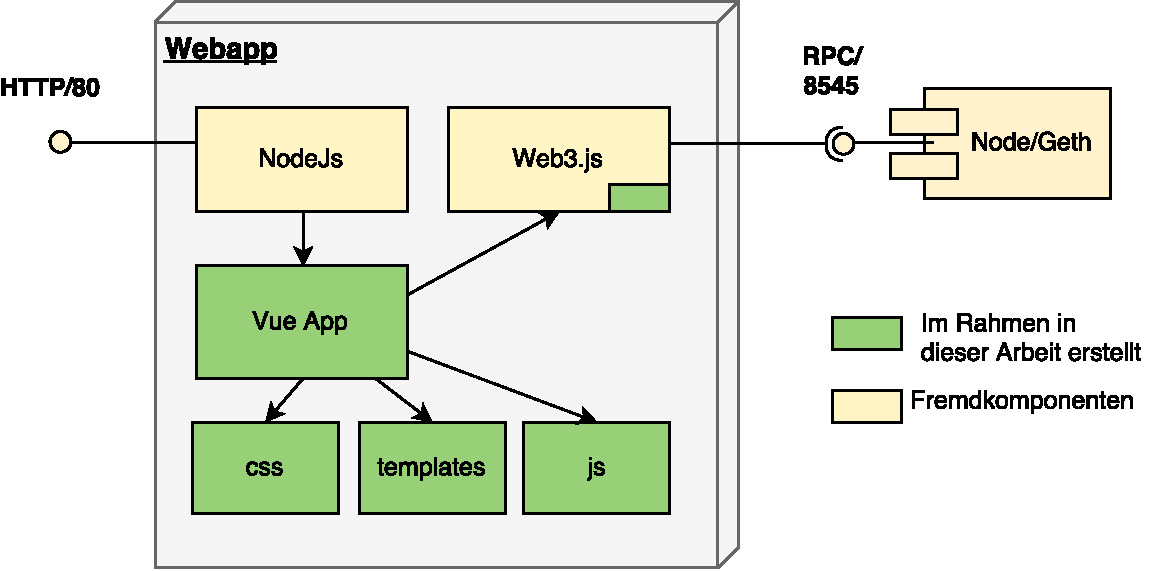
\includegraphics[width=.95\textwidth]{Aufbau_Webapp}
\caption{Aufbau der Webapp}
\label{fig:Aufbau der Webapp}
\end{figure}

\paragraph{}
Die Webapp ist eine Single Page Aplication (SPA), basiert auf \emph{NodeJS} und benutzt \emph{VueJS}\footnote{\url{https://vuejs.org/}} mit Material Design für die Benutzeroberfläche. Um mit der Blockchain zu interagieren wird die \emph{Web3.js} Library verwendet, welche die \emph{RPC/8545} Schnittstelle des \emph{Geth Nodes} implementiert. 
Die Schnittstelle gegen Aussen ist \emph{HTTP/80}. Diese ist ungeschützt und wird bei der Installation der Webapp durch einen Webserver geschützt. Die Abbildung \ref{fig:Aufbau der Webapp} zeigt eine grobe Übersicht über die verschiedenen Elemente.


\subsubsection{Webapp Abhängikeiten}
Nachfolgend ist die Liste aller zur Laufzeit benötigten Module und Libraries.

\begin{table}[H]
\centering
\caption{Webapp Runtime Abhängigkeiten}
\label{tbl:Webapp Runtime Abhängigkeiten}
\begin{tabular}{@{}lll@{}}
\toprule
Library/Modul         & Version & Beschreibung
\\ \midrule
material-design-icons & 3.0.1 & Offizielle Icons für Material Design                       \\
mdi                   & 1.9.33 & Community Icons für Material Design                       \\
moment                & 2.18.1 & Javascript Datum und Zeit Library                         \\
qrcode-reader         & 1.0.0  & Library zum Dekodieren von QR-Codes                       \\
vue                   & 2.2.2  & Vue.js                                                    \\
vue-material          & 0.7.1  & Material Design Komponenten für Vue.js                    \\
vue-resource          & 1.3.1  & Resource Management für Vue.js                            \\
vue-router            & 2.3.0  & Routing für Vue.js                                        \\
vue-toasted           & 1.0.27 & Zum Anzeigen von Status- und Fehlermeldungen              \\
vuex                  & 2.3.1  & Zentralisiertes State Management für Vue.js               \\
vuex-localstorage     & 1.0.0  & Zur Speicherung der Session im Local Storage des Browsers \\
web3                  & web.js & Library für die Kommunikation in die Blockchain           \\ 
\bottomrule
\end{tabular}
\end{table}


\subsubsection{Webapp Projektstruktur}
Die Projektstruktur ist durch die Verwendung von \emph{NPM} gegeben. Nachfolgend wird kurz eine Übersicht über die Verzeichnisse gegeben.

\begin{minipage}{\textwidth}
\begin{lstlisting}[style=tree,caption={Projektstruktur der Webapp}]
webapp
├── build                   # Build Verzeichnis
├── certs                   # Zertifikate
│   ├── server.crt
│   └── server.key
├── config                  # Konfiguration für dev/prod/test
├── debian                  # Konfiguration für das Debian Paket
├── index.html              # Hauptseite
├── node_modules            
├── package.json            # Definiert Build Process und Abhängigkeiten
├── README.md               
├── src                     # Sourcen
│   ├── App.vue
│   ├── components          # Enthält all Komponenten, Views, etc.
│   ├── main.js
│   ├── router              # Definiert das Routing
│   ├── services            # Enthält Web3 Abstraktionsservice
│   └── store.js            
├── static
│   ├── lokkit_icon_100.png
│   └── lokkit_icon_400.png
├── test                     
│   ├── e2e
│   └── unit
└── web3.js                 # Gepatchtes Web3.js
\end{lstlisting}
\end{minipage}

\subsubsection{Ethereum Node}
Die Vorbedingung zur Verwendung der Webapp ist eine laufende und korrekt konfigurierte Ethereum Node, die die jsonrpc Schnittstellen \emph{eth}, \emph{shh}, \emph{personal} auf dem Port 8545 zur Verfügung stellt.


\subsubsection{Webapp Funktionalität und Design}
Die Oberfläche kann grundsätzlich in vier verschiedene Ansichten unterteilt werden. Die erste Ansicht zeigt das Menu zur Navigation zwischen den Ansichten (vgl. Abbildung \ref{fig:4 Ansichten der Webapp} (a)). Das Menu bietet neben dem Absprung auf andere Ansichten auch die Möglickeit den Account zu wechseln. Weiter kann der \emph{Local Storage} gelöscht werden, wodurch alle bereits eingescannten Rentables wieder verschwienden. Die Abbildung \ref{fig:4 Ansichten der Webapp} (b) stellt die drei bereits eingescannten Rentables in Form von einer Liste dar. 
Ebenfalls bietet die Webapp die Möglickeit an sich mit einem beliebigen Node zu verbinden. Diese Einstellung ist z.B. in der Netzwerkansicht (vgl. Abbildung \ref{fig:4 Ansichten der Webapp} (c)) untergebracht. Für jedes Rentable gibt es ausserdem eine Detailansicht, welche die Interaktion mit dem Smart Contract in der Blockchain darstellt. Über diese Ansicht, kann der Benutzer das Rentable reservieren, schliessen, öffnen und wieder zurück geben. Die Abbildung \ref{fig:4 Ansichten der Webapp} (d) präsentiert die Detailansicht.

\paragraph{QrCode Leser}
Die Webapp benötigt für das Dekodieren des QrCode Zugriff auf eine Kamera. Dieses Feature basiert rein auf dem HTML5 Standard. Es sind keine Browserplugins nötig. Dekodiert wird mit der Library "qrcode-reader". Der Ablauf ist wie folgt:

\begin{enumerate}
    \item Die Webseite öffnet einen Live-Stream der Webcam
    \item Eine Javascript-Funktion zeichnet im Sekundentakt ein Bild auf ein Canvas (HTML Element)
    \item Anschliessend kann die qrcode-reader Library das Bild im Canvas dekodieren
\end{enumerate}

Der QrCode muss eine gültige Rentable Adresse (z.B. 0xde93b2965af6a49161f597604c600af9ea07883a) enthalten. Ist dies nicht der Fall wird eine Fehlermeldung angezeigt.


\begin{figure}
\centering\small
\setlength{\tabcolsep}{0mm}	% alle Spaltenränder auf 0mm
\begin{tabular}{c@{\hspace{12mm}}c} % mittlerer Abstand = 12mm
  \frame{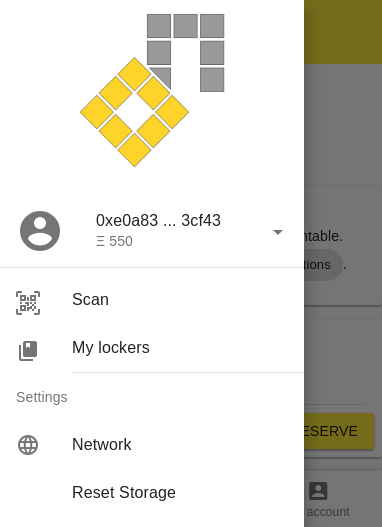
\includegraphics[width=.45\textwidth]{webapp_menu}} &
  \frame{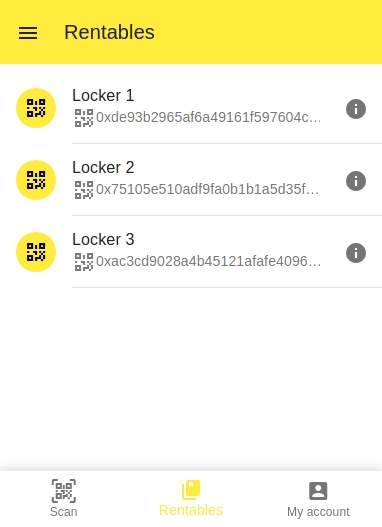
\includegraphics[width=.45\textwidth]{webapp_rentables}} \\
  (a) & (b)
  \\[.5cm]	%vertical extra spacing (4 points)
  \frame{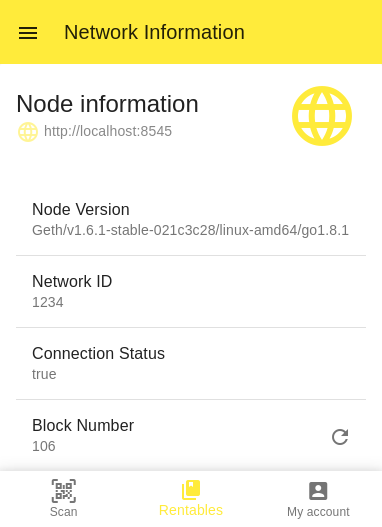
\includegraphics[width=.45\textwidth]{webapp_network}} &
  \frame{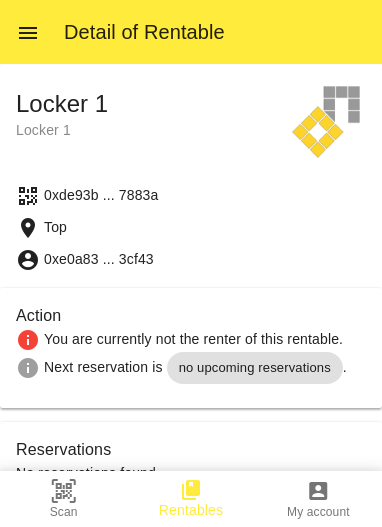
\includegraphics[width=.45\textwidth]{webapp_rentable1}} \\
  (c) & (d)
\end{tabular}
%
\caption{Webapp 4 Ansichten der Webapp-- 
Menu (a), Liste aller gescannten Rentables (b),
Netzwerkinformationen (c), Details eines Rentables (d).}
\label{fig:4 Ansichten der Webapp}
\end{figure}


\subsection{Android App}
\label{sys_subsec:Android_App}
Die Android App startet und administriert eine Ethereum Node mit dem Lokkit Genesis Block, um die Verwendung vom Lokkit Webapp (vgl. \ref{sys_subsec:Webapp}) auf einem Androidgerät zu ermöglichen.

Wenn die Android App das erste mal gestartet wird, wird der Lokkit Service gebunden und die Activity nach einem Passwort für den Account gefragt (vgl. \ref{fig:android_sequence_start}). Bei nachfolgenden Starts wird der erstellte Account geladen und die Activity nach dessen Password gefragt. Wenn die Verbindung erfolgreich hergestellt werden konnte, wird das Webapp geladen.

\begin{figure}[H]
\centering\small
\setlength{\tabcolsep}{0mm}	% alle Spaltenränder auf 0mm
\begin{tabular}{c@{\hspace{12mm}}c} % mittlerer Abstand = 12mm
  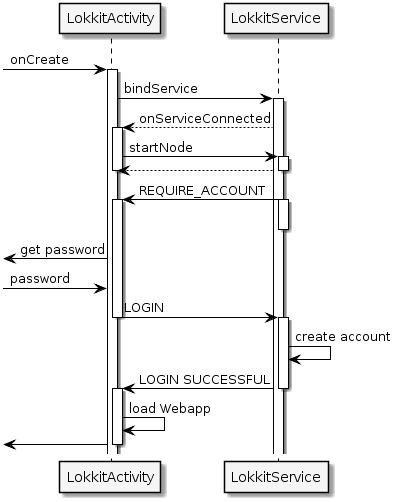
\includegraphics[width=.48\textwidth]{android_sequence_start_new} &
  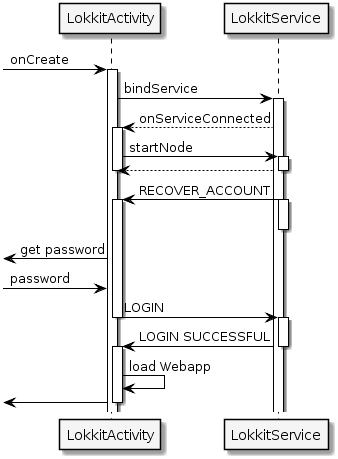
\includegraphics[width=.42\textwidth]{android_sequence_start_existing} \\
  (a) & (b)
\end{tabular}
%
\caption{erster Start (a), spätere Starts (b)}
\label{fig:android_sequence_start}
\end{figure}

\subsubsection{Statusgo}
Diese Subkomponente implementiert das Ethereum Protokoll und weitere Funktionalität von status-im. Die API kann über die statische Klasse \emph{Statusgo}\footnote{Im Paket com.github.status\_im.status\_go.cmd zu finden} in Java verwendet werden. Diese Library implementiert das gesamte Ethereum Protokoll und die light node.\cite[wiki/Build-Process-Explained]{github.com/status-im/status-go}

\subsubsection{Lokkit Service}
Der Lokkit Service konsumiert das statusgo-android Modul. Der Service wird bei Start der Applikation gestartet und bei Beenden der Applikation gestoppt. Der Service sendet und empfängt Intents (vgl. \ref{tbl:LokktService_SendIntents}, \ref{tbl:LokktService_ListenIntents}) für die Interaktion mit der Lokkit Activity (vgl. \ref{sys_subsubsec:Lokkit_Activity}).\cite[Bound Services]{developer.android.com}

Die Statusgo Library bedingt, dass eine erstellte Transaktion zuerst durch Statusgo freigegeben wird, bevor sie in die \emph{pending transactions} von geth aufgenommen wird (vgl. \ref{sys_subsec:Geth}). Dabei weist Statusgo jeder Transaktion eine id zu. Diese id ist spezifisch für Statusgo und hat keine Bedeutung im Ethereum Protokoll.

\begin{table}[H]
\centering
\caption{Intents, die vom Lokkit Service gesendet werden}
\label{tbl:LokktService_SendIntents}
\begin{tabular}{@{}L{3cm}L{2cm}L{10cm}@{}}
\toprule
action & extras & Beschreibung \\ \midrule
io.lokkit.\newline{}TRANSACTION\newline{}\_QUEUED\newline{} & id, from, to, value, gas, gasPrice & Wird versendet, wenn eine neue Transaktion von Statusgo erhalten wurde. Diese muss mit io.lokkit.COMPLETE\_TRANSACTION oder io.lokkit.DISCARD\_TRANSACTION bestätigt werden. \\\midrule
io.lokkit.\newline{}COMPLETE\newline{}\_TRANSACTION\newline{}\_FAILED & id, reason & Wird als Antwort auf io.lokkit.COMPLETE\_TRANSACTION gesendet, wenn eine Transaktion nicht bestätigt werden konnte. \\\midrule
io.lokkit.\newline{}COMPLETE\newline{}\_TRANSACTION\newline{}\_SUCCESSFUL & id & Wird als Antwort auf io.lokkit.COMPLETE\_TRANSACTION gesendet, wenn eine Transaktion erfolgreich bestätigt werden konnte. \\\midrule
io.lokkit.\newline{}LOGIN\newline{}\_SUCCESSFUL & - & Wird als Antwort auf io.lokkit.LOGIN gesendet, wenn das in io.lokkit.LOGIN gesendete Password für das Entsperren des gespeicherten Accounts verwendet werden konnte. \\\midrule
io.lokkit.\newline{}RECOVER\newline{}\_ACCOUNT & address, mnemonic & Wird gesendet, wenn der Service beim Start einen Account findet. Muss mit io.lokkit.LOGIN beantwortet werden. \\\midrule
io.lokkit.\newline{}REQUIRE\newline{}\_ACCOUNT & - & Wird gesendet, wenn ein Account gefunden wurde. Muss mit io.lokkit.LOGIN beantwortet werden. \\\midrule
io.lokkit.\newline{}COMPLETE\newline{}\_TRANSACTION & id & Da der Demonstrator nur die Lokkit webapp bedient, wurde der Einfachheit halber diese Funktionalität umgangen, indem der Service die Nachfrage nach de Account sich selbst beantwortet. \\
\bottomrule
\end{tabular}
\end{table}

\begin{table}[H]
\centering
\caption{Intents, die vom Lokkit Service verarbeitet werden}
\label{tbl:LokktService_ListenIntents}
\begin{tabular}{@{}L{3cm}L{2cm}L{10cm}@{}}
\toprule
action & extras & Beschreibung\\ \midrule
io.lokkit.\newline{}COMPLETE\newline{}\_TRANSACTION & id, password & Bestätigt die Transaktion mit id id durch Verwendung des momentanen Accounts (vgl. Statusgo.Login()) und des angegebenen Passworts. Die Transaktion wird erst durch Senden dieses Intents in die Liste der pending transactions aufgenommen. Aufruf wird bestätigt durch einen Intent mit action io.lokkit.COMPLETE\_TRANSACTION\_SUCCESSFUL, falls erfolgreich oder io.lokkit.COMPLETE\_TRANSACTION\_FAILED falls nicht erfolgreich. \\\midrule
io.lokkit.\newline{}DISCARD\newline{}\_TRANSACTION  & id           & Verneint die Transaktion mit id id. Diese Funktionalität kann verhindern, dass ohne Erlaubnis des Benutzers eine Transaktion von einer DAPP ausgelöst wird. Aufruf wird nicht bestätigt.\\\midrule
io.lokkit.\newline{}LOGIN & password     & Meldet den persistierten Benutzer an. Aufruf wird bestätigt durch einen Intent mit action io.lokkit.LOGIN\_SUCCESSFUL, falls erfolgreich oder io.lokkit.RECOVER\_ACCOUNT falls nicht erfolgreich.
\\ \bottomrule
\end{tabular}
\end{table}

\subsubsection{Lokkit Activity}
\label{sys_subsubsec:Lokkit_Activity}
Wenn die Lokkit App gestartet wird, wird die Lokkit Activity geöffnet. Diese Activity dient dazu, die Interaktion des Benutzers mit dem Lokkit Service sicherzustellen. Falls der Lokkit Service Eingaben benötigt, wird die Activity benachrichtig und wird dementsprechend den Benutzer nach der Eingabe fragen, bspw. wenn ein Passwort für einen neuen Account angegeben werden muss (vgl. \ref{fig:sys_android_new_account}).

\begin{figure}[H]
\centering
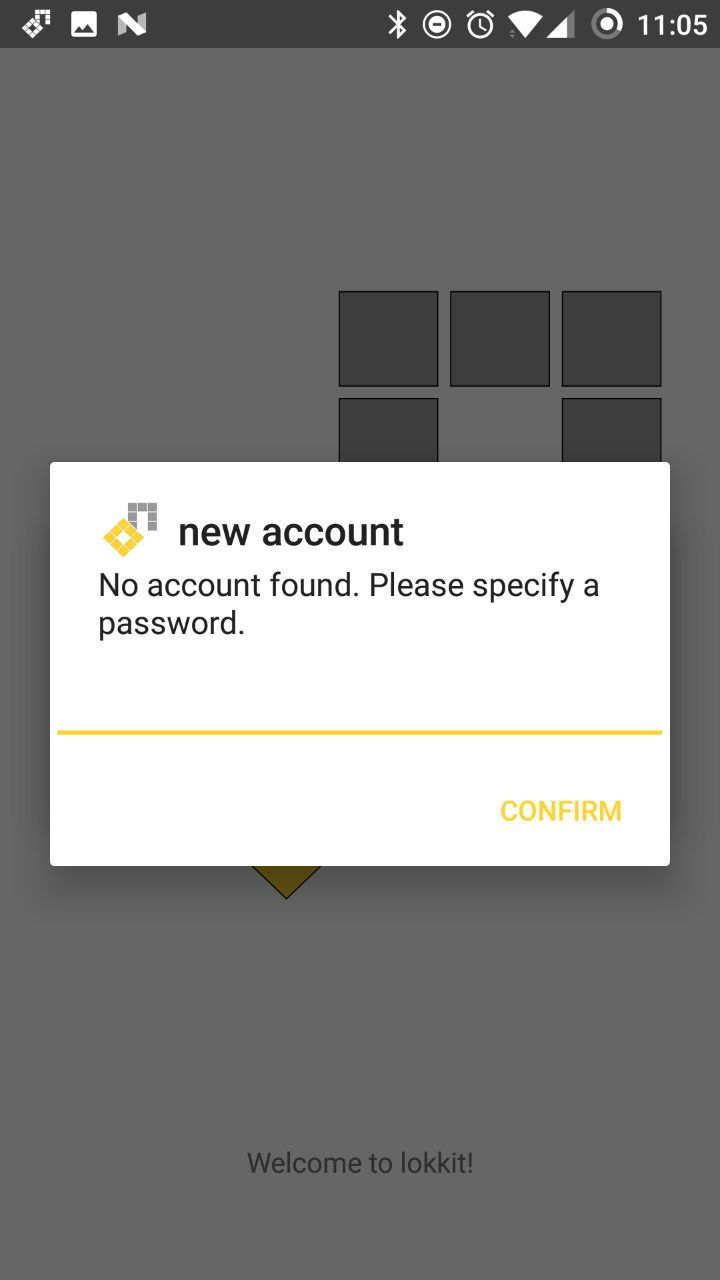
\includegraphics[width=.40\textwidth]{android_new_account}
\caption{Beispielansicht: Activity fragt den Benutzer nach einem Passwort für einen neuen Account}
\label{fig:sys_android_new_account}
\end{figure}



\subsection{Doorman}
Doorman verbindet auf eine ethereum node, die die shh und eth Protokolle enabled hat und hört auf Whisper v5 Nachrichten für die in der Konfiguration definierten Rentables. Wenn die payload der Nachrichten der Definition in der Real-Time Kommunikationsschnitstelle (vgl. \ref{sys_subsec:Real_Time_Kommunikationsschnittstelle}) entsprechen, wird ein Script ausgeführt, das als Parameter die Adresse des Rentables, sowie das command (vgl. \ref{sys_subpara:Command}) erhält.

\subsubsection{Konfiguration}
\label{sys_subsec:Doorman_Konfiguration}
Die Konfiguration des Doorman wird aus einer yml Datei\footnote{https://fdik.org/yml/} gelesen. Die Datei besitzt einen root mit Namen \emph{doorman} und Attribute für die Ethereum Node, verwendete Rentable Smart Contract Adressen und auszuführendes Script bei Erhalt einer validen Nachricht.
\begin{lstlisting}[language=yml,caption={Beispielkonfiguration für Doorman}]
doorman:
    node_ip: 127.0.0.1
    node_rpc_port: 8545
    rentable_addresses:
        - "0xf16801293f34fc16470729f4ac91185595aa6e10"
        - "0x298345dddd494c51061da2ae137df3129ce14b69"
    script: open_close_device.bat
\end{lstlisting}

\paragraph{node\_ip}
Die Url der Ethereum Node, zu der eine Verbindung aufgebaut werden soll. Diese Node muss das shh Protokoll und auch die shh API aktiviert haben (vgl. \ref{para:Whisper}). Die Adresse ist als IP anzugeben. Informationen zum Protokoll wie \emph{http://} sind auszulassen.
\paragraph{node\_rpc\_port}
Der Port, auf dem Doorman zu der Ethereum Node verbinden soll. Der Standardport ist 8545.
\paragraph{rentable\_address}
Die Adressen der Smart Contracts vom typ Rentable (vgl. \ref{sys_subsubsec:Rentable}), auf deren Nachrichten gehört werden sollen. Wird eine ungültige Rentable Adresse angegeben, werden die Befehle nicht ausgeführt.
\paragraph{script}
Das script, das ausgeführt werden soll.

\subsection{Controllers}
\subsubsection{Nuki}
\subsubsection{Schloss Marke Eigenbau}
